\chapter{LITERATURE STUDY}
\label{chap:literaturestudy}

% Ubah bagian-bagian berikut dengan isi dari tinjauan pustaka

This chapter will explain the supporting theories that are used as references for this study.
The theories described in this chapter will be presented in a systematic order, starting from the most basic
to deeper explanations.

\section{Pose Estimation}
\label{sec:poseestimation}

% Contoh input gambar
\begin{figure}[ht]
  \centering

  % Ubah dengan nama file gambar dan ukuran yang akan digunakan
  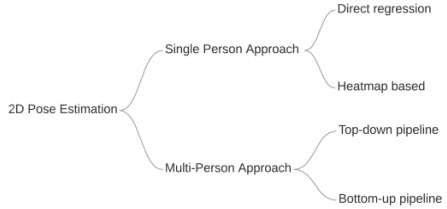
\includegraphics[scale=1]{gambar/taxonomy-pose-estimation.png}

  % Ubah dengan keterangan gambar yang diinginkan
  \caption{Taxonomy of pose estimation approaches}
  \label{fig:pose-estimation}
\end{figure}

Pose estimation is a heavily explored area with applications in gaming, animation, action recognition, activity tracking, and augmented reality.
In order to improve pose estimate outcomes, various approaches have been developed. These methods may generally be split into: Single-person and Multi-person approaches, 
as depicted in figure \ref{fig:pose-estimation}. The single-person approach is fundamentally a regression issue because it just determines the pose of a single person in an image, 
the person's position and an implicit number of keypoints are already known. However, the multi-person approach tries to solve an unconstrained problem because we do not know 
the positions and number of persons within the image \parencite{romeo}.

The single-person approach is divided into two frameworks based on the keypoint prediction method: directly regressing keypoints from the features (i.e. direct regression based framework)
or by generating heatmaps and inferencing keypoints via heatmap (i.e. heatmap based framework) \parencite{romeo}.
A direct regression-based framework can be implemented in various ways: as done by \parencite{toshev2014}, 
they presented DeepPose where their model uses a simple architecture with a convolutional layer, followed by a dense layer that will produce keypoint values in \emph{(x,y)}.
Other authors \parencite{carreira2015} suggested a technique that iteratively improves model output by feeding back mistake predictions, leading to a notable improvement in accuracy.

Then for a heatmap based framework, an alternative method can be used to generate heatmaps of all keypoints in the image
rather than directly predicting them. The final stick figure is then created using additional techniques to know the connection between keypoints or joints.
In \parencite{chen2014}, authors proposed a graphical model with pairwise
relations to make adaptive use of local image measurements. Later on, both the detection of joints and the prediction of their relationships can be accomplished using those local image measurements.
\parencite{newell2016} designed a \emph{"stacked hourglass"} network, that is closely similar to encoder-decoder architecture and is based on the sequential phases of pooling and upsampling.
They demonstrated the importance of repeated bottom-up, top-down processing with intermediate supervision for enhancing the effectiveness of human pose detection.

The multi-person approach is a more complex task because
the positions and number of persons within the image are unknown, therefore the framework has to detect keypoints and assemble an unknown number of persons. To overcome this task,
two pipelines have been proposed: top-down pipeline and bottom-up pipeline \parencite{romeo}.
Beginning with the detection of every person present in an image, the top-down pipeline creates bounding boxes. The following action uses each of the identified bounding boxes and applies a single-person method. 
For each person that is discovered, the single-person technique will generate keypoints, and then, as shown in Figure \ref{fig:top-down-approach}, the pipeline may include extra steps of post-processing and improving final results.

\begin{figure}[ht]
  \centering
  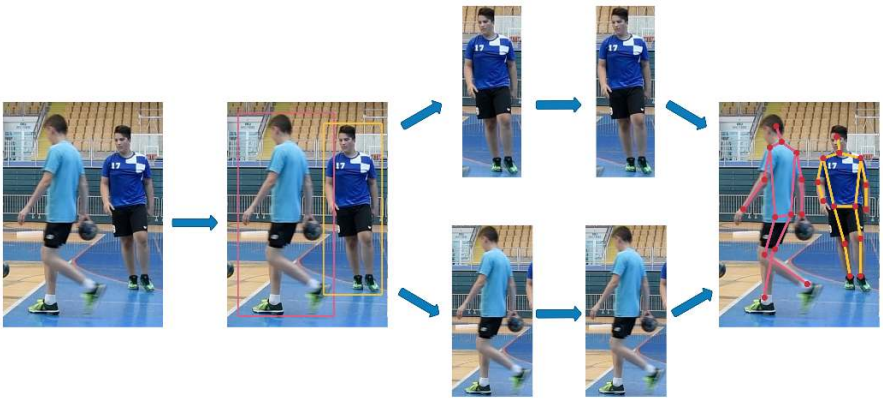
\includegraphics[scale=0.8]{gambar/top-down-approach.png}
  \caption{The top-down pipeline in multi-person approach for pose estimation}
  \label{fig:top-down-approach}
\end{figure}

Compare to a top-down pipeline, the bottom-up pipeline operates in reverse. The bottom-up pipeline begins by finding all of the keypoints, which are then connected to human instances, as seen in Figure \ref{fig:bottom-up-approach}. 
The bottom-up pipeline is probably quicker than the top-down pipeline because it doesn't detect human bounding boxes and runs pose estimation for each person individually.

\begin{figure}[ht]
  \centering
  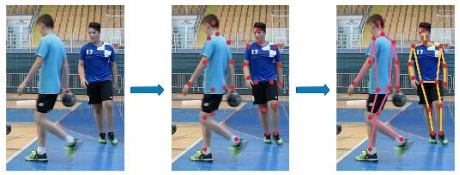
\includegraphics[scale=1.2]{gambar/bottom-up-approach.png}
  \caption{The bottom-up pipeline in multi-person approach for pose estimation.}
  \label{fig:bottom-up-approach}
\end{figure}

\section{Human Pose Estimation}
\label{sec:humanposeestimation}

Estimating human poses is one of the most challenging things in computer vision, which aims to determine the position or spatial location of certain points of a person's body (body parts/joints) from a given image or video.
Essentially it is a way to capture a set of coordinates by defining the human body joints like wrist, shoulder, knees, eyes, ears, ankles, and arms, which is a key point in images and videos that can describe a pose of a person. Then, when an image or video is given to the pose estimator model as input, it identifies the coordinates of these detected body parts and joints as output and a confidence score showing the precision of the estimations.
For many years, the main topic of discussion for numerous classical object detection applications has been the detection of persons.
With recent developments in machine-learning algorithms, computers can now understand human body language by performing pose detection and pose tracking. It has now reached a point where the hardware requirements to operate and the detection accuracy make them commercially viable.
Several industries, including security, business intelligence, health and safety, and entertainment, will be profoundly impacted by human pose estimate. Autonomous driving is one such application where this method has already shown its viability. Computers can sense and predict pedestrian behavior far more comprehensively with the use of real-time human pose detection and tracking, allowing for more consistent driving.

Pose estimation on humans can be divided into two techniques: 2D Pose Estimation and 3D Pose Estimation.
2D pose estimation is a type of pose estimation that can estimate the locations of the body joints in 2D space relative to input data (i.e., image or video frame). The location is represented with X and Y coordinates for each key point. On the other hand, 3D pose estimation transforms a 2D image into a 3D object by estimating an additional Z-dimension to the prediction. 3D pose estimation enables us to predict the accurate spatial positioning of a represented person or thing.

In the early days, the pose estimation job was treated as a part-based inference task, and there were two general groups of models. The first one is called appearance models, where features of body parts are first extracted by feature descriptors like Histogram of Oriented Gradient then distinct body parts are combined together.
Another group of models is deformable models or structural models. 
The performance of estimation models rapidly increases after deep convolutional networks are used for pose estimation. Researchers initially concentrate primarily on a well-cropped single-person posture estimate problem, which is a simplified sub-task. These days, more difficult situations, including pose estimation in a crowd, have become hot subjects thanks to the success of the more general multi-person pose estimation \parencite{song2021}.

\subsection{OpenPose}
\label{subsec:openpose}

OpenPose is a widely adopted and influential open-source library developed by Carnegie Mellon University and Intel. It aims to provide accurate and robust human pose estimation by detecting and tracking body keypoints in images and videos.
OpenPose utilizes a specific architecture where an input image is processed through a state-of-the-art CNN, such as VGG-16 or VGG-19. This CNN produces multidimensional tensors known as feature maps. These feature maps are then fed into two branches in Stage-1.
The first branch generates confidence maps for different body parts. The second branch produces part affinity maps (PAFs), which are directional vectors representing the orientations of various body limbs.
Following Stage-1, the confidence maps, PAFs, and feature maps from the CNN are combined and used as input for Stage-2. Stage-2 is a replicated version of Stage-1 and aims to refine the output further. In the OpenPose architecture, it is possible to have multiple Stage-2 stages if there are sufficient computational resources available. This can result in more accurate predictions of the human pose \parencite{cao2019}.
Figure \ref{fig:openpose-architecture} shows OpenPose network architecture, where block that predicts affinity fields that encode part-to-part association, shown in blue, and detection confidence maps, shown in beige.

\begin{figure}[ht]
  \centering
  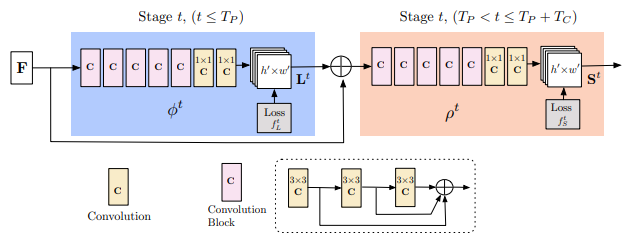
\includegraphics[scale=1.1]{gambar/openpose_architecture.png}
  \caption{OpenPose Architecture.}
  \label{fig:openpose-architecture}
\end{figure}

\subsection{MediaPipe Pose}
\label{subsec:mediapipepose}

MediaPipe Pose is a powerful open-source library developed by Google, designed for real-time human pose estimation. It utilizes machine learning models and computer vision techniques to accurately detect and track human body landmarks, enabling a wide range of applications in fields such as robotics, sports analysis, healthcare, and augmented reality. 
Over the years, MediaPipe Pose has seen significant advancements, both in terms of accuracy and performance. Recent updates have focused on improving the library's speed, allowing real-time pose estimation even on resource-constrained devices. These optimizations include model compression techniques, network architecture enhancements, and efficient implementation on hardware accelerators. Furthermore, MediaPipe Pose now supports multi-person pose estimation, enabling the detection and tracking of multiple individuals simultaneously.
In this study, MediaPipe Pose was employed to attain estimates of 2D human joint coordinates in each image frame. It builds pipelines and processes cognitive data in the form of video using Machine Learning. MediaPipe Pose uses a BlazePose that extracts 33 2D landmarks on the human body as shown in Figure \ref{fig:mediapipe-landmark}. BlazePose is a lightweight machine learning architecture that achieves real-time performance on mobile phones and PCs with CPU inference.
When using normalized coordinates for pose estimation, we should be multiplied by the width or height of the image to get the real pixel value.

\begin{figure}[ht]
  \centering
  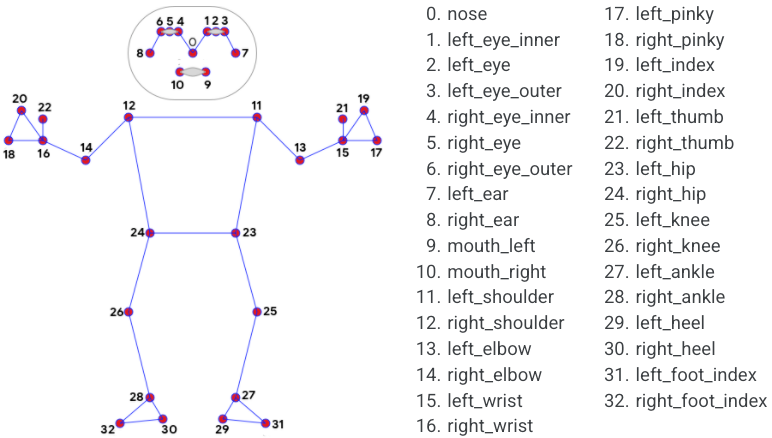
\includegraphics[scale=0.4]{gambar/mediapipe_landmark.png}
  \caption{Definition of landmarks in MediaPipe Pose.}
  \label{fig:mediapipe-landmark}
\end{figure}

BlazePose consists of two main components: detector and tracker. The detector is responsible for detecting the presence of a person in an input image or video frame. It locates the person's body within the image and provides an initial set of pose keypoints, in other words, it locates the pose region of interest (ROI) within the frame.
The detector utilizes a convolutional neural network (CNN) architecture to extract features from the input and make predictions about the presence and location of the person's body. The tracker subsequently predicts all 33 pose keypoints from this ROI. Note that the detector is run only on the first frame for video use cases. For subsequent frames we derive the ROI from the previous frame's pose keypoints \parencite{url:BlazePose}.

\subsection{YOLO-pose}
\label{subsec:yolopose}

YOLO-pose is a single-shot approach like other bottom-up approaches. However, it does not use heatmaps. Rather, it associates all keypoints of a person with anchors. Figure \ref{fig:YOLO-pose-architecture} illustrates the overall architecture with keypoint
heads for pose estimation. The most advanced detector human in terms of complexity and accuracy is YOLOv5. Consequently, they choose it as their foundation and build upon it.
The primary focus of YOLOv5 is the recognition of 80 class COCO objects, with the box head predicting 85 elements per anchor. There are three anchors of various shapes for each grid location \parencite{maji2022yolopose}.

\begin{figure}[ht]
  \centering
  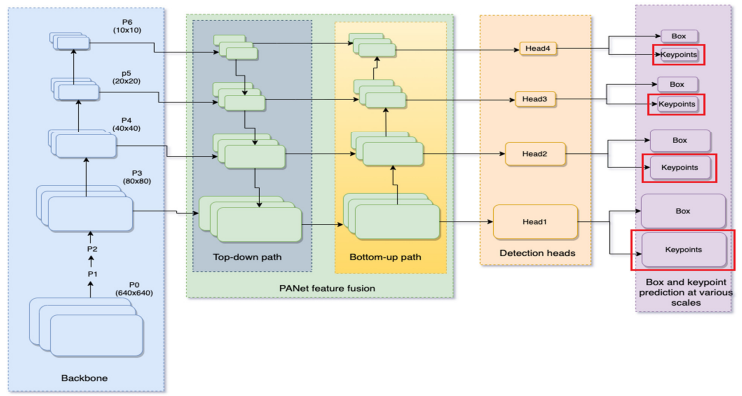
\includegraphics[scale=1.01]{gambar/yolo-architecture.png}
  \caption{YOLO-pose architecture.}
  \label{fig:YOLO-pose-architecture}
\end{figure}

For human pose estimation, it comes down to a single-class person detection problem with each person having 17 associated keypoints, each of which is again identified with a location and confidence: \emph{{x, y, conf}}.
Therefore, there are a total of 51 elements for the 17 keypoints associated with an anchor. As a result, the keypoint head predicts 51 elements and the box head predicts six elements for each anchor.
For an anchor with n keypoints, the overall prediction vector is defined as:
\begin{equation}
  \label{eq:yoloresult}
  P_v = \bigl\{ C_x, C_y, W, H, box_{conf}, class_{conf}, K_x^1, K_y^1, K_{conf}^1, ..., ..., ..., K_x^n, K_y^n, K_{conf}^n \bigr\}
\end{equation}
Keypoint confidence is trained based on the keypoint's visibility flag. Ground truth confidence is assigned to one if a keypoint is either visible or occluded. Otherwise, if it is outside of the field of view, confidence is set to zero.
YOLO-Pose uses CSP-darknet53 \parencite{wang2020} as backbone and PANet \parencite{liu2018} for fusing features of various scales from the backbone.
The Input image is passed through darknetcsp backbone that generates feature maps at
various scales \{P3, P4, P5, P6\}. PAnet is used for fusing these feature maps across multiple scales and the output is fed to detection
heads. Finally each detection head branches into box head and keypoint head \parencite{maji2022yolopose}.


\section{Humanoid Robot Pose Estimation}
\label{sec:humanoidrobotposeestimation}

Humanoid robots and people have similar shapes, which has both advantages and disadvantages. On the one hand, this allows us to start with approaches already in use for people, but on the other, it makes it harder for us to distinguish between people and humanoid robots \parencite{amini2021}.
As explained in Section \ref{sec:poseestimation}, in general, the effort to tackle the problem of pose estimation is vary depend on the number of persons (single-person or multi-person), for multiple persons can be categorized as a top-down or bottom-up approach.
In the top-down approach, the initial stage is to identify specific individuals, and the subsequent step is to implement pose estimation. The fact that the model's performance is closely associated with the performance of the person detector is one of the drawbacks of this approach. Although the state-of-the-art (SOTA) results are derived from this type of approach,  the runtime of such approaches is negatively affected by the number of persons present,
as a single-person pose estimator is run for each detection. Since the computational cost grows linearly as the number of users increases, performance is frequently not real-time \parencite{amini2021}.

Bottom-up techniques, on the other hand, are less reliant on the number of people in the image because they simultaneously identify body joints and classify them into individuals. Accurately grouping the detected keypoints in real-time is one of the bottom-up method's fundamental issues.
Recent methods arrange the identified keypoints into distinct instances using a greedy algorithm. In addition, compared to the top-down method, the bottom-up method's effectiveness is more influenced by the various scales of the people in a given image. Previous research has relied on high-resolution input size \parencite{papandreou2018} or the scale search method \parencite{cao2019} to address this issue. However, the inference time is growing as a result of these strategies.
A time-efficient method predicting keypoints at higher resolution was introduced by Cheng et al. \parencite{cheng2020}, narrowing the performance gap between bottom-up and top-down models.

There are three Pose Estimation Models for humanoid robots that we retrained with the
new dataset. Two of them use a bottom-up approach and one uses a top-down approach. For a detailed explanation of each model is located in following section.

\subsection{NimbRo's Model}
\label{subsec:nimbromodel}

NimbRo's model chose to use a similar architecture with NimbRo-Net and NimbRo-Net2 because it had such positive outcomes.
Their model, an encoder-decoder network, takes an RGB image with dimensions of \emph{w x h}. Rather than use the decoder to create a powerful feature extractor, they observe it is more required to use a deeper encoder.
A pre-trained ResNet model \parencite{he2016} is used as the encoder, and the last fully connected and global average pooling layers have been removed.
The first layer is a 7 x 7 convolutional with stride 2, followed by a max-pooling layer.  The remaining four modules of the encoder network are residual blocks, which have lower resolutions and higher depths as the number of modules rises.
Depending on the ResNet architecture that was chosen, each residual block is made up of two or three convolutional layers, followed by batch normalization, ReLU activation, and a shortcut connection. Early layers have more fine-grained spatial information,
while final layers contain more semantic information that network has extracted \parencite{amini2021}.

\begin{figure}[ht]
  \centering
  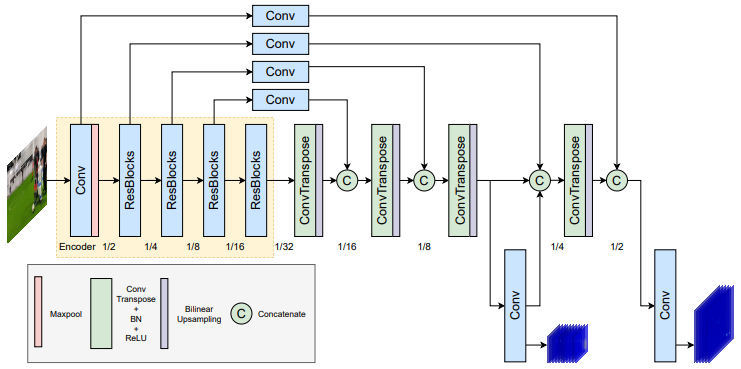
\includegraphics[scale=1]{gambar/nimbro-architecture.png}
  \caption{NimbRo's model architecture}
  \label{fig:nimbro-model-architecture}
\end{figure}

In the decoder part, they use lateral connections from different parts of the encoder, which enables the model to keep high-resolution information. They apply 1 x 1 convolution to generate a fixed number of channels for every lateral connection.
The decoder network has a feature pyramid structure involving four modules. The output from the preceding level is fed into a 3 x 3 transposed convolution at each level of the pyramid, followed by a bilinear upsampling to produce a fixed number of higher-resolution features.
The features from the corresponding lateral connection are concatenated with the features from the upsampled samples. ReLU and batch normalization are used like in the encoder, to obtain the module's final output.
As depicted in Figure \ref{fig:nimbro-model-architecture}, the model predicts heatmaps of both keypoints and limbs for scale 1/4 and only
heatmaps of keypoints for scale 1/2, where each scale is supervised with an intermediate loss \parencite{amini2021}.
For evaluation metrics, they use Object Keypoint Similarity (OKS) metric from COCO keypoint dataset \parencite{ronchi2017}.
The OKS metric is robust to the number of visible keypoints since it gives equal weight to robot instances with various quantities of visible keypoints.
The evaluation metrics they used are as follows: AP (the mean average precision over 10 OKS thresholds = [0.50:0.05:0.95]), AP50
(AP at OKS threshold = 0.50), AP75, APM for medium scale robot instances, APL for large scale instances, and AR (the mean of average recall over 10 OKS thresholds) \parencite{amini2021}.

\subsection{Keypoint RCNN}
\label{subsec:rcnn}

The architecture of Keypoint RCNN resembles the Mask-RCNN. They just differ in the output size, and the way the keypoints are encoded in the keypoint mask. Mask R-CNN itself is extended on the basis of Faster R-CNN,
in addition to the shared backbone network and FPN (Feature Pyramid Networks), it in parallel adds a new branch for predicting the object mask on the bounding box recognition branch.
The network can also be simply expanded to carry out additional tasks, including Keypoint RCNN for Person Keypoint Detection. The keypoint head of Keypoint R-CNN is very similar to the mask head of Mask R-CNN. The mask head obtains an output resolution of
28 x 28 through four 3 x 3 convolutional layers with a channel of 256 which is followed by an up-sampling layer, and finally
employ a convolutional layer to make its dimensions consistent with the object category. On the other hand, the keypoint head gets an output resolution of 56 x 56 through eight 3 x 3 convolutional
layers with 512 channels and followed by two upsampling layers \parencite{zhang2021}.
The full Keypoint RCNN architecure can be seen in Figure \ref{fig:keypoint-rcnn-architecture}.

\begin{figure}[ht]
  \centering
  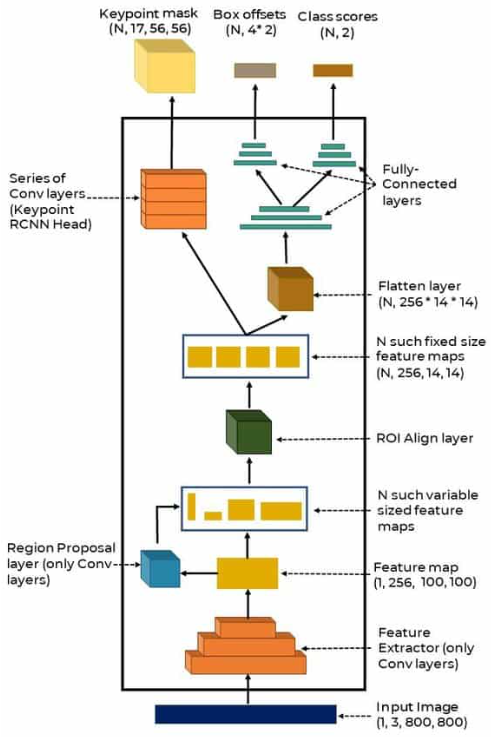
\includegraphics[scale=0.8]{gambar/keypoint-rcnn-arch.png}
  \caption{Keypoint RCNN Architecture}
  \label{fig:keypoint-rcnn-architecture}
\end{figure}


\section{Robot Operating System 2 (ROS 2)}
\label{sec:ros2}

Robot Operating System (ROS) is an open source robotics middleware that is used to assist the development of existing systems on robots. The main feature of ROS is the design of the system where data received or sent to each component in the robot is abstracted with hardware abstraction.
Given this, the existing algorithm in a program can be used on different robots, regardless of differences devices in each robot. 
To enable hardware abstraction, ROS uses a graph architecture that allows a node to communicate with other nodes over the same topic. In ROS, the hardware abstraction is formed by using a topic that has the same name and data structure that represents the type of component that a robot has.
Later, each existing node can receive or send data through the topic, regardless of how or where the data sent comes from \parencite{fikri2021}.

In ROS there are various kinds of tools that are already available to help develop existing systems on robots such as command-lines that help in program debugging, dynamic parameter configuration when the program is running, visual monitoring of internal data on the robot, and so on. In addition, with the existing package management in ROS, everyone can use existing packages or add new packages to facilitate the further development of a robot, without the need to create
reset the entire system as needed. The second generation of the Robot Operating System, ROS 2, is a continuation of ROS which brings reliability and performance for real-time use of robots while still supporting the features of the previous ROS \parencite{Maruyama}. Unlike its predecessors, which use TCPROS/UDPROS as the communication system used at each node, ROS 2 uses Data Distribution Service (DDS), an industry standard for real-time communication systems and end-to-end middleware. 
With the use of DDS, ROS 2 will focus more on the use of middleware in the field of robotics, while low-level communication between each node will be returned to the DDS implementation that is used \parencite{fikri2021}.

\subsection{ROS 2 Node}
\label{subsec:ros2node}

ROS 2 nodes are the main component of the graph architecture in ROS 2. ROS 2 nodes are generally used to represent a single process in a robot, such as accessing motors, processing images, and so on. Each existing node can later communicate with other nodes in two ways, as shown in Figure \ref{fig:ros2node}, a node with a publisher can send data via a topic which will then be channeled to other nodes with subscribers connected to that topic.
In addition, a node with a service client can also send a data request via a service which will later be processed and sent back in the form of a response data by another node that has a service server connected to the service.
The communication process between existing nodes will be carried out in an abstract manner, where a node will send data to a topic or service, regardless of whether the data will be received by other nodes or not. Each node will only need to send data to the topic or service with the appropriate name and interface type so that the data can be sent in an abstract manner to other nodes \parencite{fikri2021}.
Apart from topics and services, ROS 2 also recognizes another communication channel between nodes known as an action. But because this study does not use it, we will not discuss it further.
\begin{figure}[ht]
  \centering
  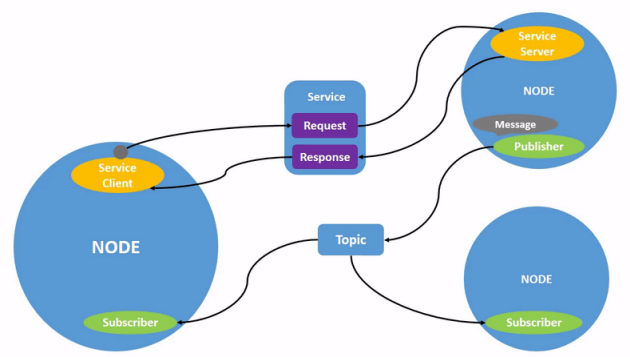
\includegraphics[scale=1]{gambar/ros2_node.png}
  \caption{Communication diagram between nodes through topics and services in ROS 2}
  \label{fig:ros2node}
\end{figure}

\subsection{RQt}
\label{subsec:rqt}

RQt is a Qt-based GUI framework that is used to implement tools in managing nodes in ROS 2. RQt has relatively the same function as ROS 2 CLI, which is for debugging purposes on existing communication systems in ROS 2, but this RQt works visually in GUI form. In RQt, there are several standard tools that can be used to do various things such as viewing image data visually, viewing communication relationships between nodes in the form of diagrams, and so on.
As shown in Figure \ref{fig:rqtgraph}, RQt has a tool called rqt graph (ROS Graph) which can be used to see the relationships that exist at each node in the form of topics, services, and actions.
In addition to the standard tools that have been provided, the GUI-based tools on RQt can also be made by yourself or modified according to the desired needs. These changes can be made through a plugin made specifically for RQt. Later the plugin can be embedded in the RQt tools that were developed and can be used directly to access the existing communication system in ROS 2 \parencite{fikri2021}.
\begin{figure}[ht]
  \centering
  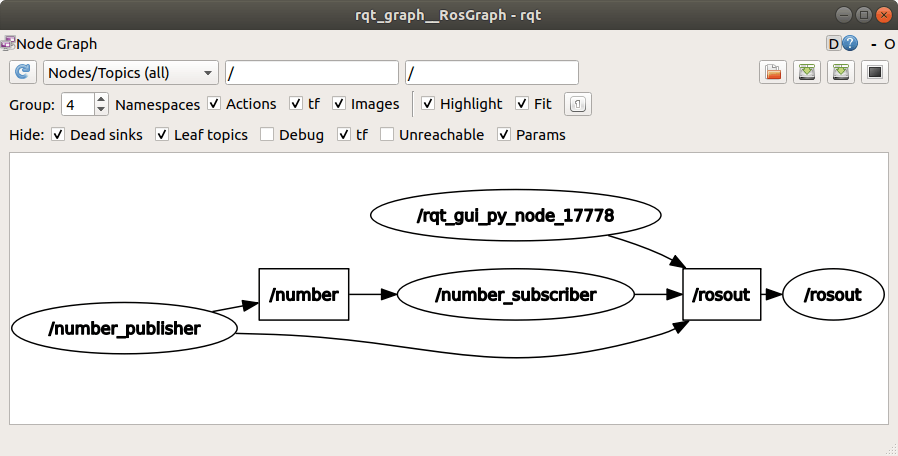
\includegraphics[scale=0.45]{gambar/rqt_graph.png}
  \caption{Example view of rqt graph (ROS Graph)}
  \label{fig:rqtgraph}
\end{figure}